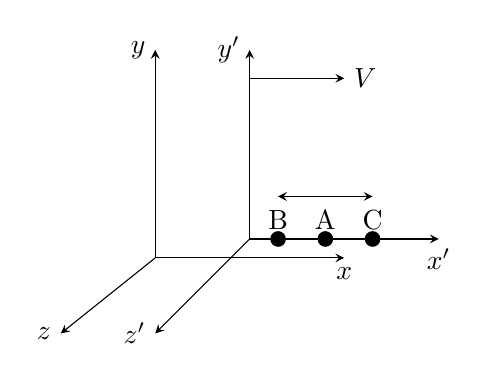
\begin{tikzpicture}[>=stealth,scale=1.2]

% Assi principali (sistema non primato)
\draw[->] (0,-0.2,0) -- (2,-0.2,0) node[below] {$x$};
\draw[->] (0,-0.2,0) -- (0,2,0) node[left] {$y$};
\draw[->] (0,-0.2,0) -- (-1,-1,0) node[left] {$z$};

% Assi primati
\draw[->] (1,0,0) -- (3,0,0) node[below] {$x'$};
\draw[->] (1,0,0) -- (1,2,0) node[left] {$y'$};
\draw[->] (1,0,0) -- (0,-1,0) node[left] {$z'$};

% Velocità V
\draw[->] (1,1.7,0) -- (2,1.7,0) node[right] {$V$};

% Punti
\node[circle,fill,inner sep=2pt] (B) at (1.3,0) {};
\node[circle,fill,inner sep=2pt] (A) at (1.8,0) {};
\node[circle,fill,inner sep=2pt] (C) at (2.3,0) {};

\node[above] at (B) {B};
\node[above] at (A) {A};
\node[above] at (C) {C};

% Frecce attorno ad A
\draw[<->] (1.3,0.45) -- (2.3,0.45);

\end{tikzpicture}